\section{Mergeable Priority Queue ADT}

Mergeable priority queue is a type of priority queues that support all the operations of a regular priority queue, in addition to the operation \proc{Union}

$\proc{Union}(A,B)$: returns a new priority queue containing all elements from $A$ and $B$. As a precondition, we may assume that $A$ and $B$ are disjoint.

Some implementations of a mergeable priority queue may also support the operation \proc{Decrease-Priority} and \proc{Delete}.

\section{Binomial Heap}

In this section, we will examine a data structure that implements the mergeable priority ADT. It supports all operations in $\Theta(\log n)$ time.

\begin{definition}[Binomial Tree]
    The binomial tree $B_k$ of degree $k$ is defined recursively as follows:
    \begin{itemize}
        \item $B_0$ consists of 1 node;
        \item $B_k$ consists of two binomial trees of degree $k-1$, where the root of one of the trees is made the first child of the root of the other.
    \end{itemize}
\end{definition}

\begin{figure}[htbp]
    \centering
    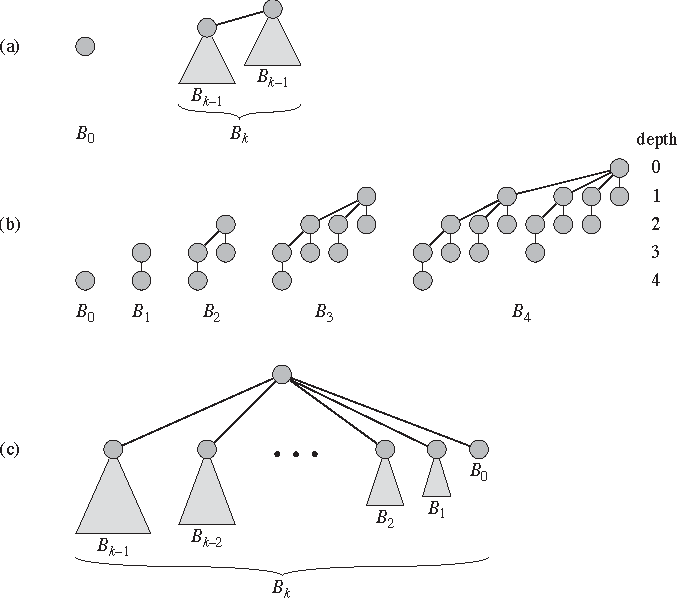
\includegraphics[width=0.8\linewidth]{binheap/binheap.pdf}
    \caption{(a) The recursive definition of binomial tree; (b) Binomial trees of degree 0-4; (c) Binomial heap viewed as rooted tree}
    \label{fig:binheap}
\end{figure}

A binomial tree $B_k$ of degree $k$ has $2^k$ nodes, and there are $\choose{k i}$ nodes at depth $i$ for all $i = 0,\ldots,k$. The root of $B_k$ has $k$ children, each of which is a root of a binomial tree. The subtree rooted at the $i$th child is $B_{k-i}$. In other words, the children of the root of $B_k$ are the roots of $B_{k-1},\ldots,B_{0}$ in order from left to right.

Each node, in addition to its key, stores its degree, pointer to its parent, pointer to its leftmost child, and pointer to its next sibling.

\begin{figure}[htbp]
    \centering
    \includegraphics[width=0.7\linewidth]{binheap/binheap-pointers.pdf}
    \caption{Pointers in a binomial tree.}
    \label{fig:binheap-pointers}
\end{figure}

A binomial heap is a linked list of binomial trees with increasing large degree such that each binomial tree satisfies the priority condition (i.e. the priority of a node is less than or equal to the priority of its parent). The next sibling field of the root of the binomial trees are used to link the binomial trees together into this linked list.

There is at most one binomial tree of each degree in a binomial heap. 

A binomial heap with $n>1$ elements has at most $\lceil \log_2 n \rceil$ binomial trees. If $n$ is a power of 2, then a binomial heap with $n$ nodes consists of 1 binomial tree. For example, a binomial heap with 27 nodes consists of 4 binomial trees.
$$
B_0 \to B_1 \to B_3 \to B_3 \qquad \Leftarrow \qquad \left({\underbrace{1}_{B_4} \underbrace{1}_{B_3} \underbrace{0}_{\text{nothing}} \underbrace{1}_{B_1} \underbrace{1}_{B_0}}\right)_2 = 27
$$

\section{Operations on Binomial Heap}

\subsection{Linking Two Binomial Trees}

Linking 2 binomial trees of the same degree is easy because linking $B_k$ and $B_k$ simply gives a new binomial tree of degree $k+1$. More specifically, we update the first child pointer and the degree of the root at one tree, and chagne the parent pointer and next sibling pointer of the root of the other tree. The linking operation takes $O(1)$ time.

\begin{codebox}
    \Procname{$\proc{Binomial-Link}(y,z)$}
    \li $\attrib{y}{parent} = z$
    \li $\attrib{y}{sibling} = \attrib{z}{child}$
    \li $\attrib{z}{child} = y$
    \li $\attrib{z}{degree} = \attrib{z}{degree} + 1$    
\end{codebox}

\subsection{Union Two Binomial Heaps}

To union two binomial heaps, we need to merge the two linked lists sorted by degree. We link the roots of equal degrees in increasing order until at most 1 root of each degree remains. This is somewhat similar to the merge step in merge sort and analogous to \textbf{addition of binary numbers}.

For example, starting with two linked lists of binomial trees
$$
B_0 \to B_1 \to B_3 \to B_4 \qquad B_0 \to B_1 \to B_3 \to B_4 \to B_5
$$
$$
B_0 \to \boxed{B_1 \to B_1} \to B_3 \to B_3 \to B_4 \to B_4 \to B_5
$$
$$
B_0 \to B_2 \to \boxed{B_3 \to B_3} \to B_4 \to B_4 \to B_5
$$
$$
B_0 \to B_2 \to B_4 \to \boxed{B_4 \to B_4} \to B_5
$$
$$
B_0 \to B_2 \to B_4 \to \boxed{B_5 \to B_5}
$$
$$
B_0 \to B_2 \to B_4 \to B_6
$$

If the first binomial heap $H_1$ consists of $h_1$ trees and $H_2$ consists of $h_2$ trees. In the worst case, we need to merge $O(h_1+h_2)$ binomial trees, each of which takes $O(1)$ time. After each link operation, the number of trees in the list decreases by 1, so there can be at most $h_1+h_2-1$ link operations. Therefore, the overall runtime of \proc{Union} is $O(h_1+h_2) \leq O(\log n)$.

The actual implementation of \proc{Union} is a little bit complicated as we need to consider a few different cases.

\begin{codebox}
    \Procname{$\proc{Union}(H_1,H_2)$}
    \li $H = \textbf{new } \proc{Binomial-Heap}()$
    \li $\attrib{H}{head} = \proc{Merge}(H_1,H_2)$ \RComment{same as \proc{Merge} in mergesort}
    \li \If $\attrib{H}{head} \isequal \const{nil}$ \Then
        \li \Return $H$
        \End
    \li $\id{prev-x} = \const{nil}$
    \li $x = \attrib{H}{head}$
    \li $\id{next-x} = \attrib{x}{sibling}$
    \li \While $\id{next-x} \neq \const{nil}$ \Do
        \li \If $\attrib{x}{degree} \neq \attrib{\id{next-x}}{degree}$ \textbf{or} ($\attrib{\id{next-x}}{sibling} \neq \const{nil}$ \textbf{and} $\attribb{\id{next-x}}{sibling}{degree} \isequal \attrib{x}{degree}$) \Then
            \li $\id{prev-x} = x$
            \li $\id{x} = \id{next-x}$
        \li \ElseIf $\attrib{x}{key} \leq \attrib{\id{next-x}}{key}$ \Then
            \li $\attrib{x}{sibling} = \attrib{\id{next-x}}{sibling}$
            \li $\proc{Binomial-Link}(\id{next-x},x)$ 
        \li \Else
            \li \If $\id{prev-x} \isequal \const{nil}$ \Then
                \li $\attrib{H}{head} = \id{next-x}$ 
            \li \Else
                \li $\attrib{\id{prev-x}}{sibling} = \id{next-x}$ 
                \End
            \li $\proc{Binomial-Link}(x,\id{next-x})$
            \li $x = \id{next-x}$
        \End
        \li $\id{next-x} = \attrib{x}{sibling}$
        \End
    \li \Return $H$
\end{codebox}

\subsection{Insertion}

We can insert a new node into a binomial heap by first creating a binomial tree of degree 0, and then calling $\proc{Union}(H,H')$ where $H'$ is the newly created binomial tree. This is analogous to incrementing a binary number.

\begin{codebox}
    \Procname{$\proc{Insert}(H,x)$}
    \li $H' = \textbf{new } \proc{Binomial-Heap}(H,x)$
    \li $\attrib{x}{parent} = \const{nil}$
    \li $\attrib{x}{child} = \const{nil}$
    \li $\attrib{x}{degree} == 0$
    \li $\attrib{H'}{head} = x$
    \li $H = \proc{Union}(H,H')$  
\end{codebox}

The runtime of \proc{Insert} is $O(\log n)$.

\subsection{Getting the Minimum}

Search the list of roots to find the root with smallest priority. This takes $O(\log n)$ because $H$ has $O(\log n)$ roots.

\subsection{Extract Min}

We need to find the minimum using the procedure described just now. And we remove the tree rooted at the node $x$ with smallest priority from $H$. Let $H'$ be the binomial heap consisting of the binomial trees rooted at the children of $x$ in reverse order. We can put them back by calling $\proc{Merge}(H,H')$. Each step takes $O(\log n)$ so overall the algorithm still runs within a constant factor of logarithmic time.

\subsection{Decreasing Priority}

This is similar to the bubbling up procedure used in a normal min-heap. This operation also takes $O(\log n)$ time.

\begin{codebox}
    \Procname{$\proc{Decrease-Priority}(H,x,p)$}
    \li $\attrib{x}{key} = p$
    \li $\attrib{y}{x}$ 
    \li $z = \attrib{y}{parent}$
    \li \While $z \neq \const{nil}$ \textbf{and} $\attrib{y}{key} < \attrib{z}{key}$ \Do
        \li \textbf{swap} data in $y$ and $z$
        \li $y = z$
        \li $z = \attrib{y}{parent}$  
\end{codebox}